\chapter{Overview of the existing System}
The internship project was not focused on creating an entirely new system from scratch, but rather on a deep redesign and restructuring of an existing system developed many years ago using legacy technologies and affected by several issues and critical limitations.

Before discussing the architectural, technological, and implementation choices that were made, it is necessary to carry out a thorough analysis of the current system, in order to understand its behavior, operational flows, technologies used, the main issues to be addressed, how to resolve them, how to prevent them from reoccurring in the future, and how to ensure that the new system is scalable and maintainable.

\section{Current System Architecture}

The \textit{SRP} system is fundamentally divided into two primary segments: 
\begin{itemize}
    \item Company Network;
    \item Client Network.
\end{itemize}

These segments interact and communicate exclusively through a \textit{DMI Console}, which acts as a unidirectional bridge, transferring requests from the client network to the internal company network. 

The overall architecture is depicted in the diagram in figure \ref{fig:as-is-system-design}.

\begin{figure}[htbp]
  \centering
  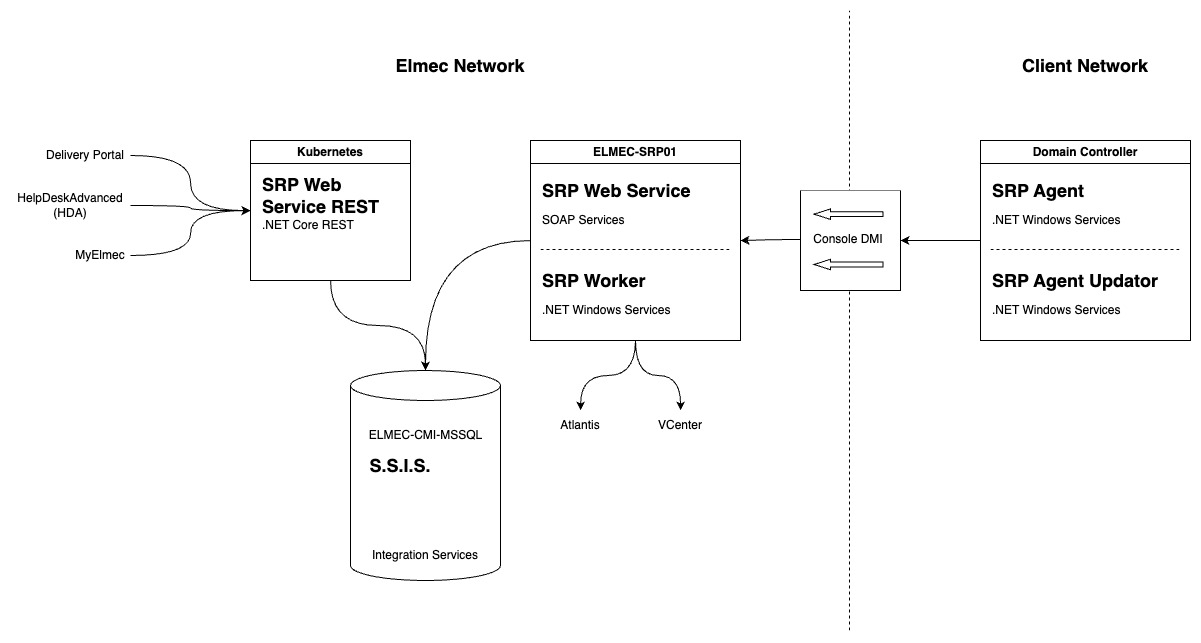
\includegraphics[width=1.0\textwidth]{images/as-is/SRP AS-IS (System Architecture).jpg}
  \caption{AS-IS System Architecture}
  \label{fig:as-is-system-design}
\end{figure}

The system's operational flow involves several key components across both networks, orchestrating the processing of service requests.

\subsection{Main Functionalities and Components}
The current \textit{SRP} system relies on a suite of interconnected components, each serving a specific role in the lifecycle of a service request.

Elmec Network Components:
\begin{itemize}
    \item \textbf{SRP Web Sevice REST}:  This component, deployed on a Kubernetes cluster, exposes .NET Core RESTful services. It serves as the primary interface for external systems such as:
    \begin{itemize}
        \item \textbf{Delivery Portal}: An asset management system used to manage Service Request catalog configuration and Elmec's internal and client servers;
        \item \textbf{HDA (HelpDeskAdvanced)}: A ticket management system. Each service request is intrinsically linked to an HDA ticket via an ID, and HDA is responsible for initiating and associating service requests with existing tickets.
        \item \textbf{MyElmec}: A client-facing portal enabling customers to create, manage, and monitor the various services provided by Elmec (e.g., servers, management software, cloud solutions).
    \end{itemize}
    The \textit{SRP Web Service REST} communicates with the \textit{ELMEC-CMI-MSSQL} server.
    \item \textbf{ELMEC-CMI-MSSQL}: This server hosts the central SQL Server Database for the SRP system. It is the persistent storage layer for all service request data and related information.
    \item \textbf{S.S.I.S. (SQL Server Integration Services)}: Running on the ELMEC-CMI-MSSQL server, SSIS packages are crucial for data transformation and import/export operations. They facilitate the transfer of data, such as master data (e.g., Active Directory users, Organizational Units, groups) sent by SRP Agents, into the database. Each SSIS package is designed to transform the received information for database insertion or vice versa.
    \item \textbf{ELMEC-SRP01}: This Windows Server functions as the core engine for service requests within the Elmec network. It houses all the PowerShell scripts associated with individual service requests, which are maintained by the Platform team. Key components residing on ELMEC-SRP01 include:
    \begin{itemize}
        \item \textbf{SRP WebServiceSoap}: This component provides SOAP services primarily for communication with the SRP Agent located on the client side. It interacts with the database to retrieve necessary information before exposing it to the agents for service request execution.
        \item \textbf{SRP InternalWorker}: A Windows service that operates similarly to the SRP Agent but executes entirely within the Elmec network. This is utilized for service requests that do not require interaction with the client's network or Active Directory (e.g., "no patch" service requests). The InternalWorker queries the database every 10 seconds for "internal worker" type jobs (like removing a server from a patching session, or resetting a managed Virtual Machine), connects to the SOAP service, retrieves the Service Request ID and its fields, and initiates job execution. It also monitors logs every 30 seconds to determine the job's status.
    \end{itemize}
\end{itemize}

The only component in the client's network is called \textbf{Domain Controller}, which represents the client's Active Directory domain controller, where the communication tools with Elmec are installed. It hosts:
\begin{itemize}
    \item \textbf{SRP Agent (.NET Windows Service)}: Typically, one agent is configured per client domain, specifically for Active Directory (AD) and Exchange-related service requests. This agent performs two main functions:
    \begin{itemize}
        \item Every 8 hours, it reads master data (AD users, OUs, groups) from the domain controller and sends it to ELMEC-SRP01 for storage via SSIS.
        \item Every 5 minutes, it queries ELMEC-SRP01 for pending Service Requests. Upon finding any, it requests detailed information, loads the corresponding PowerShell script, and executes it. After initiating the script, the agent informs ELMEC-SRP01 that the SR is "running" and proceeds to the next SR.
    \end{itemize}
    
    \item \textbf{SRP Agent Updator (.NET Windows Service)}: This service continuously monitors the SRP Agent folder for a file with a .new extension. If detected, it stops the SRP Agent, updates it, and restarts it
\end{itemize}

\subsection{Interactions and Communication between Customers and Company networks}
The Communication between the company network and the clients' networks is a critical aspect of the SRP system's operations and is handled through the \textbf{DMI Console}.

The DMI console serves as a key infrastructural component, primarily acting as a communication bridge between the customer's network and Elmec's internal network. Specifically, for the SRP system, the DMI console is responsible for transferring service requests (SR) from the customer's network to Elmec's internal network, although it does not handle traffic in the opposite direction.

\subsubsection{Operation of the DMI Console}
The connectivity of the DMI appliances to Elmec is established through multiple OpenVPN connections, initiated by the appliance towards the Brunello 4 and Mendrisio Data Centers (for Swiss customers). The DMI consoles are not directly exposed to the Internet and are accessible only by authorized personnel. Hardware requirements for a DMI node include 4 GB of RAM, 4 cores, and 50 GB of disk space.

Following recent developments in the DMI, the new consoles use K3S for container management. K3S is a lightweight, certified Kubernetes distribution designed for edge, IoT, and CI/CD environments. It is characterized by being a single binary that reduces external dependencies and uses SQLite as the default database, greatly simplifying installation and management. It already includes essential components such as \textit{containerd} \cite{k3s}.

All consoles are centrally managed via Rancher, and the deployment of the application stack is delegated to ArgoCD, which ensures that container versions are constantly updated. For security reasons, the console in the customer network by default exposes only SSH, while services such as SRP are selectively enabled and only when necessary. All application data present on the consoles is stored on a LUKS (Linux Unified Key Setup) encrypted volume\footnote{A platform-independent hard disk encryption method that can be used to encrypt disks across a wide variety of tools. This not only ensures full compatibility and interoperability between different software but also guarantees that password management occurs in a secure and documented manner \cite{luks}.}, which can only be unlocked if the VPN tunnel is established. The operating system update is performed through a standard Elmec system, called PMD (Patching Management Dashboard).

\section{Service Requests Workflow}

The lifecycle of a Service Request within the current system is orchestrated through a series of defined states and automated processes, involving interactions between various components and human operators. The flow is designed to manage SRs from initiation to completion, handling approvals, execution, and potential errors.

\begin{figure}[htbp]
    \centering
    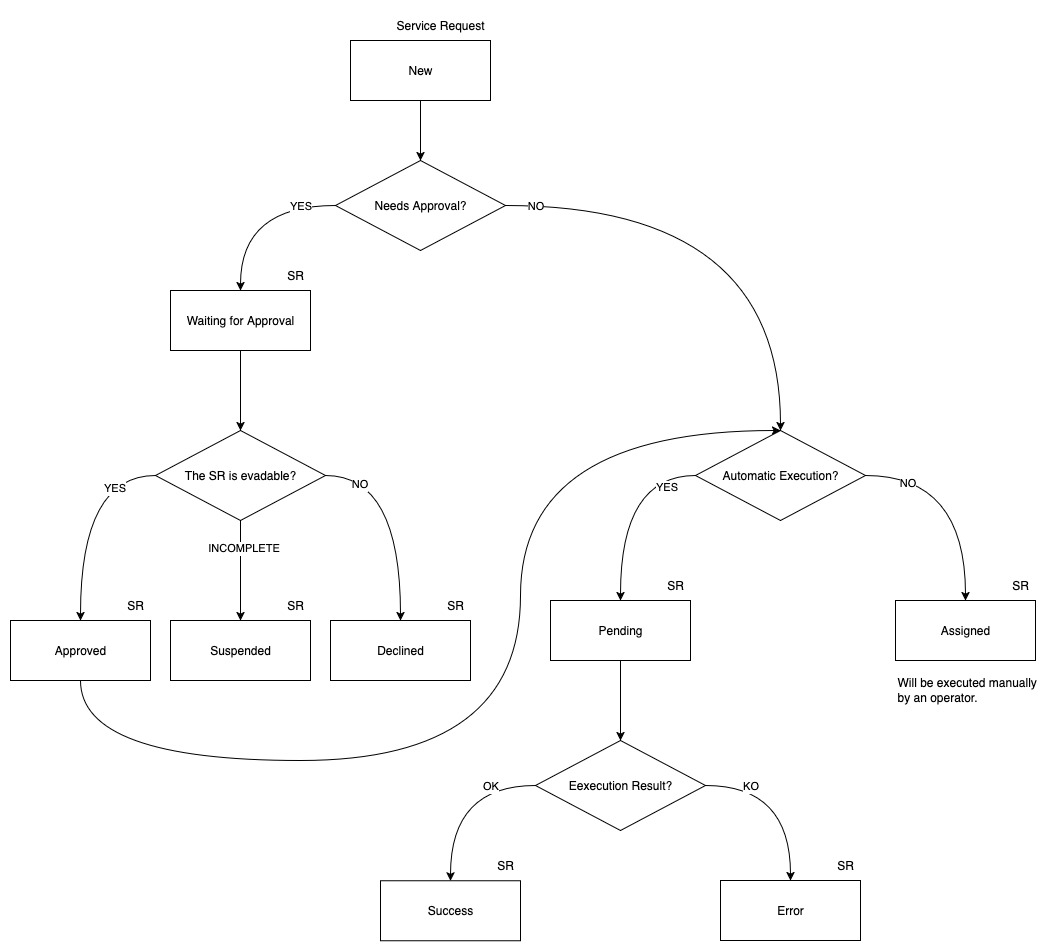
\includegraphics[width=\textwidth,keepaspectratio]{images/sr-state-diagram-simple.jpg}
    \caption{High-Level Service Request Lifecycle}
    \label{fig:sr-state-flowchart-simple}
\end{figure}


In Figure \ref{fig:sr-state-flowchart-simple} a simple and high-level flowchart is shown that illustrates the main flows and scenarios. Instead, in Figure \ref{fig:flowchart-as-is} a complete and detailed flowchart is shown that illustrates all the details about every flow, including information on the jobs and components that manage the various sections of an SR's workflow.

\begin{figure}[htbp]
    \centering
    \includegraphics[height=\textheight, keepaspectratio]{images/as-is/Flowchart AS-IS.jpg}
    \caption{AS-IS Complete Service Request Execution Workflow}
    \label{fig:flowchart-as-is}
\end{figure}

\subsection{SR Initiation and Initial State Management}
A Service Request can be initiated through two primary channels:

\begin{itemize}
    \item \textbf{Via MyElmec Portal}: Clients can submit an SR by completing a dedicated form from the MyElmec portal. Upon saving the form, a ticket is created in the HelpdeskAdvanced (HDA) system with a \texttt{QUALIFIED} status, and a corresponding Service Request is generated in SRP with a \texttt{NEW} status. These two entities are then linked via the HDA Ticket ID;
    \item \textbf{Via HDA Ticket by Elmec Operator}: Operators have the ability to associate a catalog SR directly with a ticket they are managing within the HDA interface. When the ticket is saved in a \texttt{DELEGATED} status, the SR is created in SRP with a \texttt{NEW} status, linked to the ticket, and immediately triggers the SR workflow within SRP.l
\end{itemize}

Following its creation, the system evaluates whether the Service Request requires approval by the operators. The logic for setting the initial SR and HDA ticket states is as follows:
\begin{itemize}
    \item \textbf{If approval is required}: the Service Request is set to \texttt{WAITING FOR APPROVAL} status, and the corresponding HDA ticket is set to \texttt{QUALIFIED}. A communication is added to the ticket, indicating that the SR needs validation from an operator before execution;
    \item \textbf{If no approval is required and it's linked to an automatism}: the Service Request enters a \texttt{PENDING} state, and the HDA ticket is set to \texttt{DELEGATED};
    \item \textbf{If no approval is required and it's not linked to an automatism}: the Service Request is \texttt{ASSIGNED}, and the HDA ticket is set to \texttt{PASSED}. A communication is added to the ticket, noting that the SR requires manual processing by an operator.
\end{itemize}

\subsection{Approval and Execution Workflows}
For SRs requiring approval (\texttt{WAITING FOR APPROVAL} state with an HDA \texttt{QUALIFIED} ticket), an operator's intervention is necessary to validate the request. The operator has three possible actions:
\begin{itemize}
    \item \textbf{Cancel the SR}: the HDA ticket is set to \texttt{CLOSED ABORTED}, the SR status becomes \texttt{DECLINED}, and a notification email is sent to the requesting client;
    \item \textbf{Request client modification}: the HDA ticket is set to \texttt{WAITING USER}, the SR status becomes \texttt{SUSPENDED}, and a notification email is sent to the client. The workflow pauses until the client modifies the SR via Elmec.com;
    \item \textbf{Approve the SR}: the HDA ticket is set to \texttt{DELEGATED}, and the SR status becomes \texttt{APPROVED}.
\end{itemize}

Once a SR is \texttt{APPROVED}, SRP manages its subsequent flow based on whether it is linked to an automatism:
\begin{itemize}
    \item \textbf{If the SR is linked to an automatism}: the SR transitions to a \texttt{PENDING} state, while the HDA ticket remains \texttt{DELEGATED}. This implies it's awaiting automated execution;
    \item \textbf{If the SR is not linked to an automatism}: the SR is immediately set to \texttt{ASSIGNED}, and the HDA ticket is moved to \texttt{PASSED}. A note is added to the ticket indicating that the SR requires manual processing.
\end{itemize}

An SR in \texttt{PENDING} state is awaiting the execution of its associated automatism. The outcome of this automated execution determines the next state:
\begin{itemize}
    \item \textbf{Successful execution}: the SR is set to \texttt{COMPLETED}, and the corresponding HDA ticket is set to \texttt{SOLVED};
    \item \textbf{Unsuccessful execution}: the SR transitions to an \texttt{ERROR} state, and the HDA ticket is set to \texttt{PASSED}. Communication regarding the error is added to the ticket for visibility within HDA.
\end{itemize}

The execution of Service Requests themselves can involve the SRP Agent on the client's Domain Controller for operations requiring client-side interaction (e.g., Active Directory or Exchange environment changes). The SRP Agent periodically checks \texttt{ELMEC-SRP01} for pending SRs. If found, it retrieves the SR details, loads the relevant PowerShell script, and executes it. The agent then informs ELMEC-SRP01 that the SR is running. Monitoring is performed by a scheduled READLOG task on the client side, which checks the PowerShell script's log file every minute. A "KEY" in the log indicates completion, prompting the SRP Agent to inform ELMEC-SRP01 to set the SR to COMPLETED, triggering an HDA status update. An "ERROR" key indicates failure, leading to the log being sent to ELMEC-SRP01 and an error signal. A timeout mechanism also signals an error if completion is not detected within a specified duration


\section{Problems and core issues of the current system}
The analysis of the architecture and workflow of the current SRP system has revealed a number of critical issues that compromise its scalability, maintainability, and reliability. These problems are deeply rooted in the technological and design choices made years ago and are evident across several key areas of the system, from catalog management to script execution and the import of master data from Active Directory.

\subsection{Architectural and Technological Challenges}

The SRP system is characterized by a fragmented architectural structure and complex interdependencies between its main components, which leads to several critical issues.

\subsubsection{Monolithic Frontend Component}
The user interface, responsible for navigating the Service Request catalog and completing the associated forms, is an excessively large and complex Vue.js frontend component (nearly 11,000 lines). This architecture makes modifications, extensions, and client-specific customizations exceptionally challenging. The logic for managing dynamic fields, their interdependencies, and the rules for compilation and validation are all handled at the frontend level through a long series of hard-coded conditional statements, such as the following:

\begin{minted}[linenos,tabsize=2,breaklines]{vue}
<div v-if="field.desc == 'Domain'">
    ...
</div>
\end{minted}

This, in addition to mixing business logic with presentation, represents a significant challenge for catalog configuration, as there is no centralized way to manage the fields and their relationships. Every change, therefore, requires a direct intervention on the code, making the system inflexible and difficult to maintain, especially in a context where the operator modifying the catalog is not a programmer and does not know how the frontend code is structured. For instance, if an operator wanted to add a new "Domain" field to a Service Request, this field would need to have the exact description "Domain" and type "domain"; otherwise, the Vue.js component would not render it correctly.

These dynamics make the system fragile and susceptible to frequent errors that waste time and resources for both clients and operators.

\subsubsection{Overly Generic Backend REST Service}

The only information about the fields returned by the backend REST service (\texttt{SRPWebSeviceREST}), besides the field name and its mandatoriness, is its \textit{type}. It is therefore easy to imagine how this information, which should only be an indication of the component that needs to be rendered (e.g., textbox, select, radio button, etc.), can become an identifier for something much broader.

For example, a field of type \texttt{UPN} is a composite field derived from the value of another field, '\texttt{Display Name}', concatenated with an '\texttt{@}' symbol, and suffixed with the value from a select field whose options are the client's domains, provided by an external REST service (e.g., "\texttt{n.guarini@elmec.it}", where "\texttt{n.guarini}" is the value of the "\texttt{Display Name}" field, and "\texttt{elmec.it}" is the value of the "\texttt{Domain}" select field). 

Despite this complexity, the REST service returns only a JSON document of this type:

\begin{minted}[linenos,tabsize=2,breaklines]{json}
{
    "idField": 1603,
    "descField": "UPN",
    "type": "upn",
    "mandatory": true
}
\end{minted}

thus delegating to the frontend the responsibility of interpreting the type and rendering the field correctly.

\subsubsection{Dependency on the SRP Agent}

The import of data from clients' Active Directories and the actual execution of Service Requests are handled by an agent (\texttt{SRPWindowsService}) installed directly on the clients' Domain Controllers. This approach presents several challenges:

\begin{itemize}
    \item \textbf{Security and Permissions}: The agent often requires credentials with elevated privileges (e.g., \texttt{domain-admin}), which clients are increasingly reluctant to grant.
    \item \textbf{Reliability and Control}: The configurations on the agent and the Domain Controller are complex and difficult to manage centrally, which can cause execution errors and data synchronization issues.
    \item \textbf{Scalability}: The need to install, configure, and maintain an agent for each client domain represents a significant operational effort. Alternatives such as more modern provisioning systems will be evaluated.
    \item \textbf{Obsolete Communication Patterns}: The unidirectional communication through the \textit{DMI Console} creates a bottleneck and complicates the management of asynchronous operations. Communication between components in the client's network and the company network is based on polling (e.g., the SRP Agent queries the server every 5 minutes), an approach that introduces latency and inefficiencies.
\end{itemize}

\subsection{Code and Data Management Issues}

Code and data persistence management is another critical aspect of the system, characterized by a lack of versioning and modern debugging tools.

\subsubsection{Unversioned and Undebuggable Stored Procedures}
The intensive use of Stored Procedures\footnote{Stored procedures are SQL code routines, or sets of instructions, that are pre-compiled and stored within a relational database. They act as logical units of execution, encapsulating business logic directly at the database level \cite{stored-procedures}.} in the MSSQL database represents one of the major weaknesses. These procedures contain fundamental business logic and are:
\begin{itemize}
    \item \textbf{Unversioned}: There is no centralized version control system for Stored Procedures. Changes are made directly on the database, making it impossible to track changes, revert to previous versions, or test modifications in separate environments.
    \item \textbf{Difficult to Debug}: Debugging Stored Procedures is a complex and cumbersome process, often requiring direct access and specific SQL server tools, with the risk of affecting the production environment.
\end{itemize}

\subsubsection{Inaccessible and Unversioned SSIS Jobs}
SSIS packages\footnote{SQL Server Integration Services (SSIS) is a platform for building data integration and workflow solutions. It is a key component of Microsoft SQL Server, primarily used for Extract, Transform, Load (ETL) operations, enabling the extraction of data from various sources, its transformation, and its loading into different destinations \cite{ssis}.} are essential for data import and export operations (e.g., AD master data). However, these jobs reside physically on the \texttt{ELMEC-CMI-MSSQL} server, and the only way to access and modify them is via a remote desktop. This approach prevents versioning and collaboration, limits accessibility by making maintenance and debugging an onerous and risky activity, and creates a \textit{single-point-of-failure} and a strong coupling between the import/export business logic and the infrastructure.

\subsection{Database Schema and Data Integrity Issues}

\begin{figure}[htbp]
    \centering
    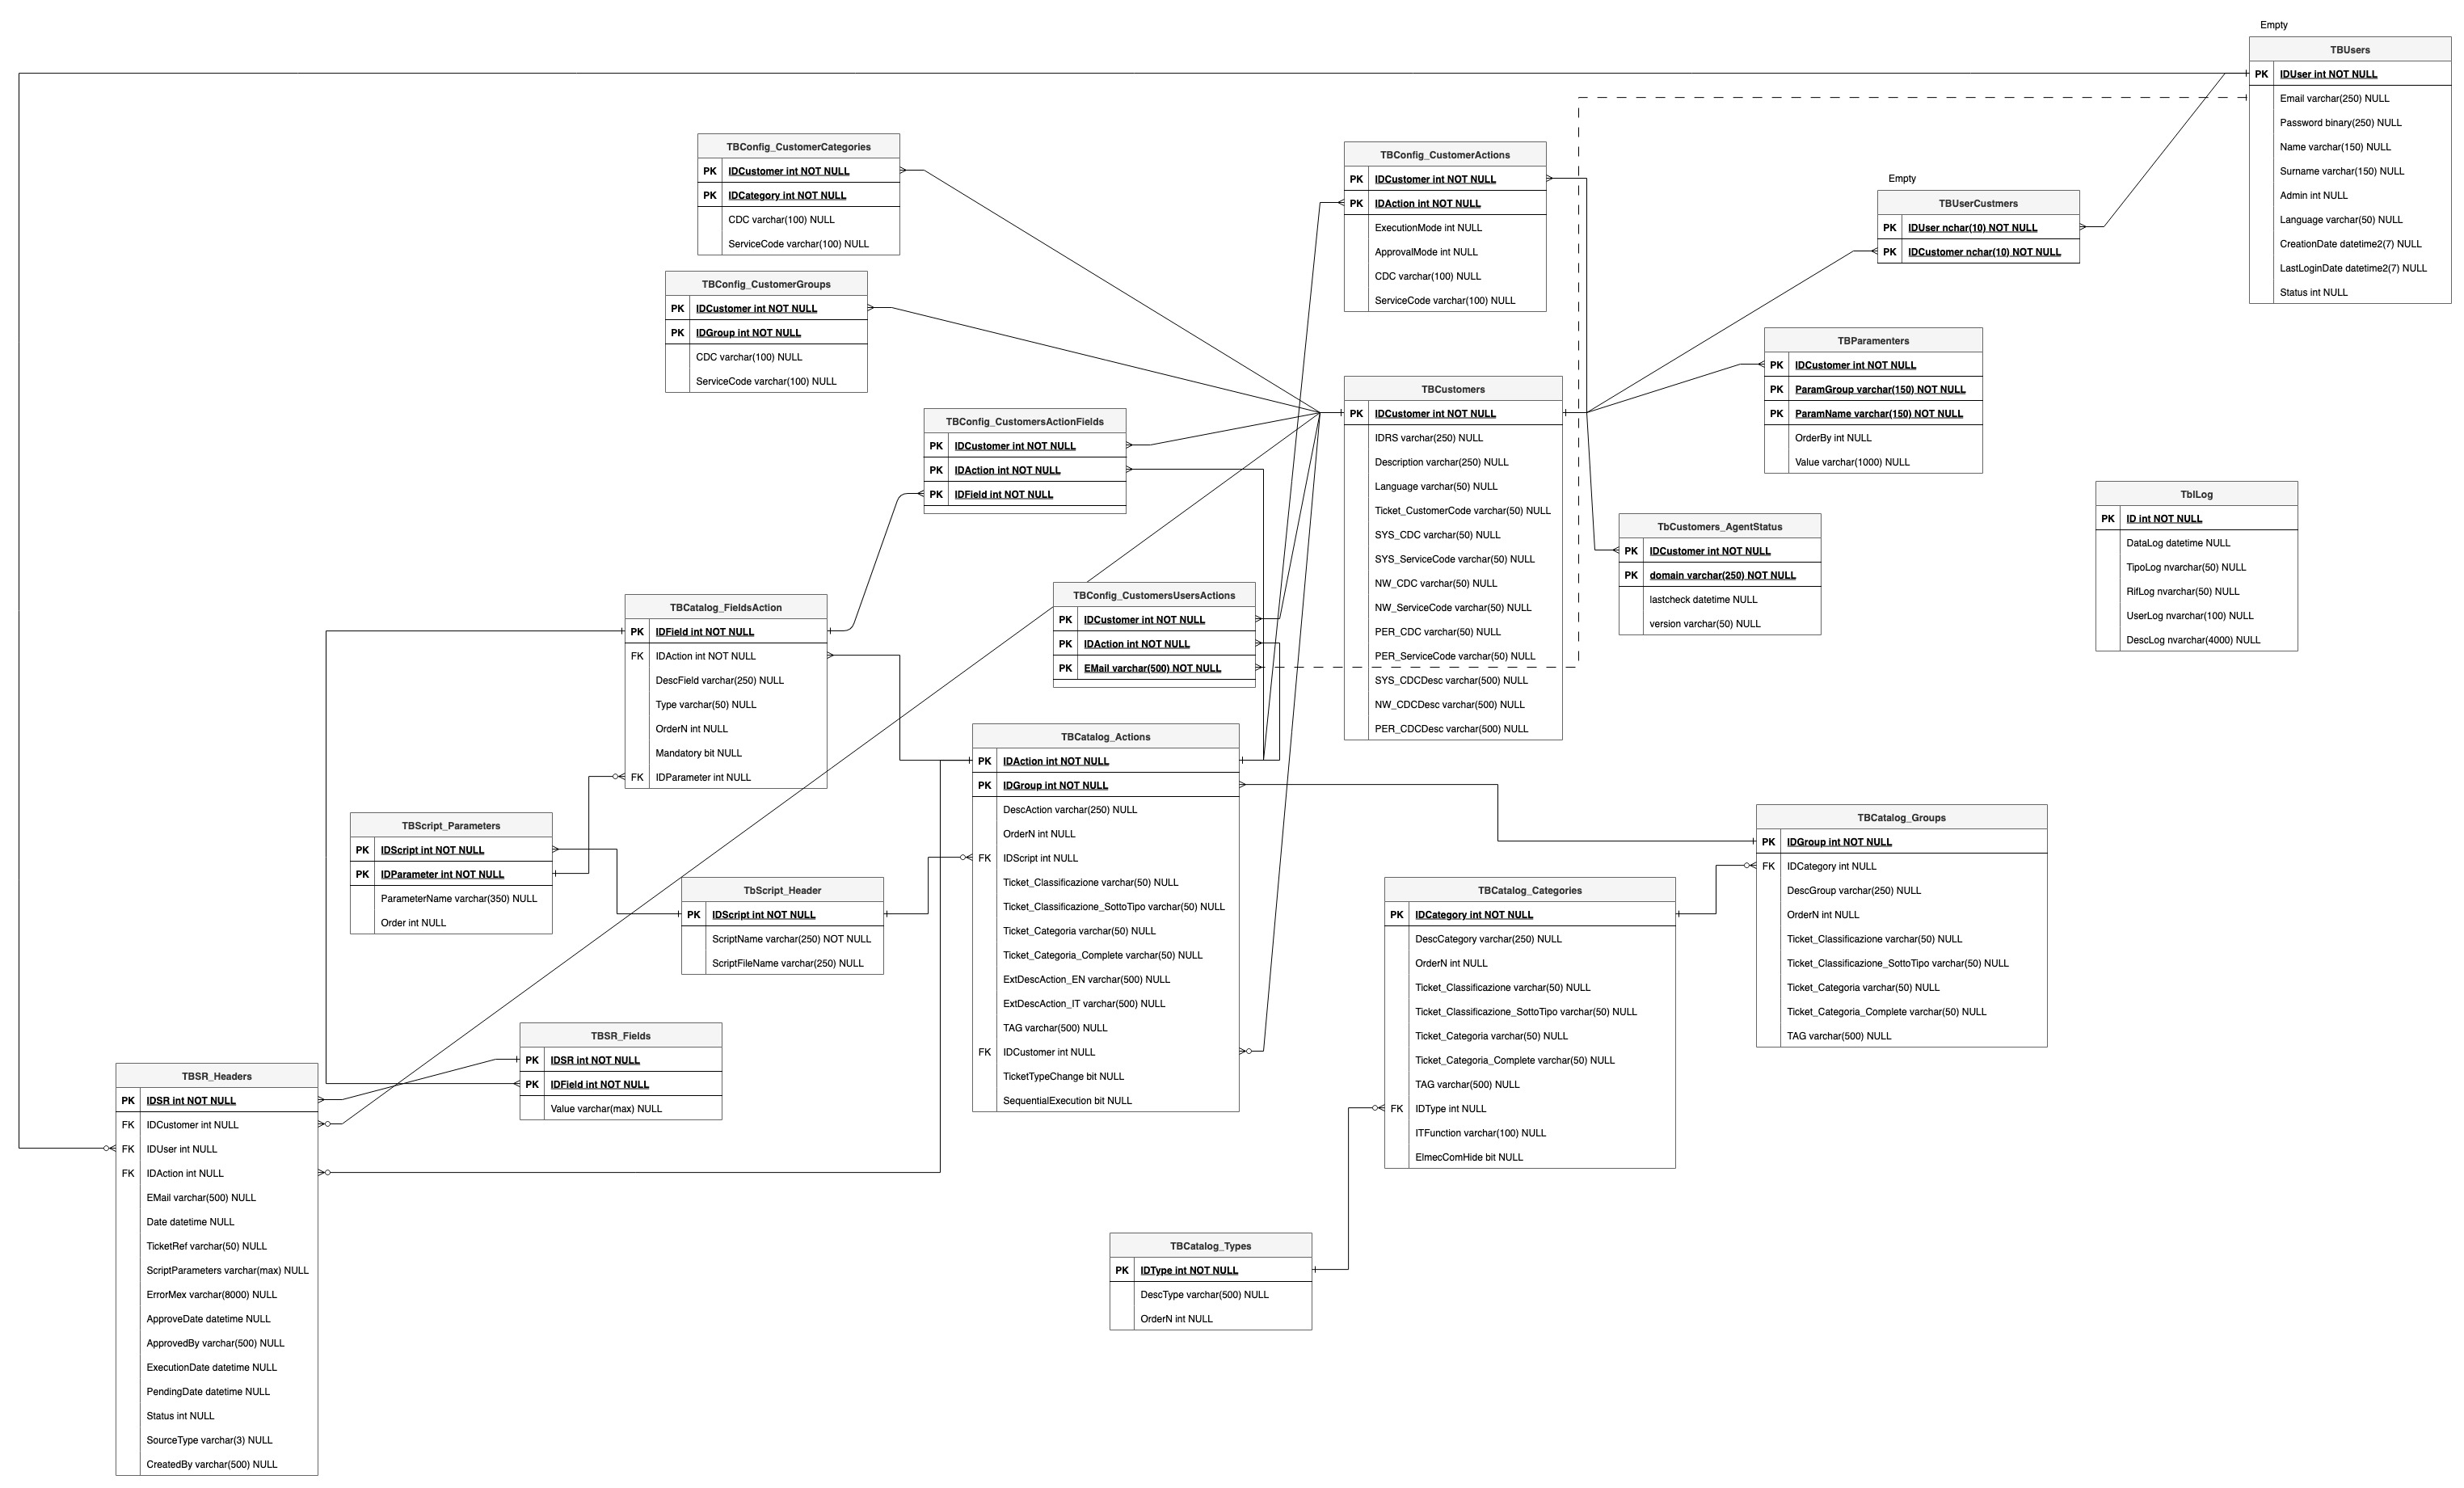
\includegraphics[width=\textwidth, keepaspectratio]{images/as-is/ER SRM-SRP AS-IS.jpg}
    \caption{AS-IS Database ER Schema}
    \label{fig:er-as-is}
\end{figure}

The analysis of the database schema, represented in figure \ref{fig:er-as-is}, has revealed a number of significant issues that affect the quality and integrity of the data managed by the SRP system.

\subsubsection{Lack of Data Integrity and Consistency}
One of the most significant problems concerns the lack of explicit referential integrity constraints. In the schema in figure \ref{fig:er-as-is}, although the relationships between tables have been inferred manually, they are not defined at the database level through the use of foreign keys. This absence prevents the database from guaranteeing data integrity: for example, a row in a child table could refer to a non-existent row in the parent table. Such a scenario, known as a "dangling reference\footnote{The "dangling pointer" is a problem typically addressed in the context of low-level programming, where a pointer refers to a memory area that is no longer valid because it has been freed or because the pointer is used outside the context of the variable's existence to which it refers \cite{apogeo-fondamenti-programmazione}, but the same dynamic can also be applied in the context of databases, where the "pointers" are represented by foreign keys.}", can generate anomalies and inconsistencies in the system, making the data unreliable and debugging extremely complex.

\subsubsection{Data Redundancy}
Another issue is the high data redundancy and the large number of duplicate attributes across different tables. This design, which deviates from the principles of normalization, leads to storing the same information in multiple locations, which not only increases the data volume but also introduces a high risk of inconsistencies.

\subsubsection{Unclear and Inconsistent Naming Conventions}
The naming convention for attributes and tables is inconsistent and unclear. The schema presents a mixture of conventions (e.g., \texttt{IDGroup} vs. \texttt{GroupID}, English names mixed with specific terms) and typos (e.g., \texttt{TBParamenters}), making it difficult to immediately understand the function of each field. In many cases, the naming is not explicit enough to describe the role of an attribute, requiring an in-depth knowledge of the system to correctly interpret the relationships and business logic. This lack of a unique and standardized vocabulary hinders collaboration among developers, complicates code maintenance, and increases the likelihood of errors.

\subsection{Maintenance and Operational Challenges}

The daily management of the system is made complex by several inefficiencies and obsolete design choices.

The current system design does not allow for the effective reuse of Service Requests and catalog configurations. Consequently, every modification or addition requires the creation of a new Service Request, even for small variations, leading to a innefficient and difficult-to-manage catalog, consisting of numerous duplicate SRs and fields. This, while functional, is not a scalable approach and leads to significant inefficiencies in catalog management itself. For example, if a Service Request needs to be modified for all clients who use it, the operator will have to modify not only the SR in question but also all the duplicate SRs for each client, with the risk of forgetting a modification or making mistakes. This approach, although probably conceived to prevent error propagation, makes the catalog difficult to navigate and maintain.

The new architecture will need to address these challenges by introducing a more robust, versioned system based on modern software design principles and patterns.